%\chapter{A Protocol for Data Provenance}
%\chapter{Computational Pipelines for Sport}
\chapter{Computational Pipelines}
\label{ch:prov}
\startchapter

The previous chapters introduced sport technologies, and looked at common techniques in the literature to analyse spatio-temporal sport data. Compared to traditional sport statistics, spatio-temporal data analysis involves sophisticated modelling to mine the data for meaningful insights. Furthermore, it is common to combine multiple spatio-temporal analysis procedures together into a computational pipeline: e.g. a preprocessing stage to correct for field shape, followed by application of a data mining algorithm to detect patterns, followed by visualisation of the results to translate these patterns into a form that humans can interpret.

This chapter lays the foundations for describing and reasoning about computational pipelines for sport analysis. Many tools are available for constructing computational pipelines (e.g. operating systems, such as Unix, provide primitive operations for constructing pipelines where the output of one program is fed as input to another). However, an important criterion for sport analysis is to be able to trace the final output (e.g. a player rating) back to the source (e.g. the events that contribute to that player rating in the video recording of the match). This ability to trace the output of a pipeline back to the original source(s) is referred to in the computer science literature as \textit{data provenance} and is the main property sought after in this chapter.

\section{Background}

% \subsection{Introduction}

\subsection{Definition of Data Provenance}

A desire to track provenance of information exists at multiple levels. In this thesis, \textit{data provenance} refers to the capture of information, either prospectively or retrospectively, to allow the traceability of data that undergoes transformations back to the original source(s). For example, a statement of the form ``dataset $Y$ was arrived at by applying transformation operation $T$ to dataset $X$''. In contrast, \textit{provenance} in the general sense is defined as the ability to trace some output back to the inputs that \textit{caused} it to occur. For example, a coach may wish to establish the provenance of a goal by tracing back the actions that contributed to it.
% [cite presentation that data prov is too general] (Done!)

The former concept of \textit{data provenance} can be formalised and solved through technological means. The latter concept of \textit{provenance}, is general and difficult to formalise. As \textit{provenance} relates to questions of causality, at a minimum, it requires a model that can be used to answer \textit{what-if} questions to establish whether an alternative value for some input would have impacted on the final output. Attempts to design data provenance systems to support this more general concept of provenance have led to it being informally declared ``an unsolvable problem''\footnote{[Presentation] Jennifer Widom, ``Panda: A System for Provenance and Data'', GoogleTechTalks. \url{https://www.youtube.com/watch?v=tprA7aOb7Is} 12:18}.

Due to the insurmountability of designing a protocol for capturing \textit{provenance} in the general sense, this chapter will focus on design of a protocol for capturing \textit{data provenance} in the stricter sense of data and the transformations applied to them. The purpose of the \textit{data provenance} system is to establish a foundation that later chapters can build on top of. Its design is influenced by the higher level \textit{provenance} questions that sport performance analysts seek to answer about the game.

\subsection{Designing for Data Provenance}

Data provenance systems can be designed systematically by considering the use-cases of queries a user wishes to ask of it \cite{Bowers2006}. Sport performance analysis can be thought of as a scientific workflow. Thus designing a data provenance system for sport performance analysis requires that the system can answer typical questions one would ask of a scientific workflow, such as which years of data were used to produce a specific graphical figure. It should also incorporate reasoning appropriate to the sport domain. For example, if a dataset includes data from games played simultaneously at different venues, the two games should be treated separately from each other for data provenance purposes to incorporate prior knowledge of physical limitations that prevent the two games from having any meaningful influence on each other. As another example, one may be able to treat certain stoppages, such as events that return the ball to a \centrebounce{} as \textit{state resets} to decouple them from past actions and thus make human reasoning simpler due to the smaller provenance chain. There may also be provenance information that should \textit{not} be tracked. For example, there may be a restriction that for player privacy, it should \textit{not} be possible to trace information back to individual players (\chref{ch:de-identification}). In such a case, the data provenance foundations need to be designed to capture provenance information to support the questions one wishes to ask, while being able to reason with partial data due to the need to hide certain details of how the data were derived.

\subsection{Data Provenance Protocols}

This section provides an overview of data provenance systems and representations proposed in the literature. It identifies W3C PROV \cite{Moreau2015} as influential in standardising the core concepts needed to represent provenance information. Recent developments attempt to increase the ease and level of detail with which one can capture provenance information.

\textbf{2005}

% displayed in \figref{fig:simmhan}
Simmhan et al. \cite{Simmhan2005} provide a taxonomy for describing data provenance systems in terms of ``use of provenance'', ``subject of provenance'', ``provenance representation'', ``storing provenance'' and ``provenance dissemination''. They outline multiple needs for provenance, including: estimating data quality; auditing; ability to replicate processes with updated inputs; attribution to ensure proper citation or for compliance with intellectual property laws; and informational reasons to allow querying the provenance to help understand the data, or to search out datasets that were produced in a particular manner (for example, when conducting a meta-review, one might limit their search to datasets that comply with a certain methodological requirements, such as having a randomised control). While their taxonomy considers the representation of provenance information, surprisingly their paper does not consider how the representation of provenance information relates to the representation of the underlying workflow. Nevertheless, many of the systems they surveyed used, either explicitly by design or implicitly through dependencies, a Directed Acyclic Graph (DAG) to represent the workflow, coupled with a provenance system that either \textit{eagerly} produces provenance information upon execution of the workflow (i.e. provenance metadata is produced as an additional artefact alongside the other data transformations), or \textit{lazily} allows determination of provenance after execution by inverting transformations (inverting transformations requires that they are analysable, thus most of the work for inverting transformations focuses on inverting standard SQL queries rather than arbitrary code).

% <!-- Their taxonomy for representation only distinguished between "annotation" (eager evaluation of provenance as the workflow is executed) and "inversion" (lazy evaluation of provenance through inversion of transformations). Many of the systems they surveyed used a Directed Acyclic Graphs (DAGs) to represent provenance. -->

% Image removed: would make obtaining all rights to distribute problematic.
% \begin{figure}[!h]
% \centering
% \includegraphics[width=\linewidth]{figs/dag/simmhan2005fig1.png}
% \caption{Taxonomy of provenance systems, copied without modification from Simmhan 2005 \cite{Simmhan2005}}
% \label{fig:simmhan}
% \end{figure}

\textbf{2006}

Bowers et al. \cite{Bowers2006} describe a provenance capture format and query mechanism for the ``Kepler'' scientific workflow system. They introduce the Read, Write, State-Reset (RWS) provenance model, a minimalistic system for capturing provenance while allowing complex workflows such as those that involve sliding time windows and recursion. Logging groups (called ``firings'' in their paper) of reads and writes allows tracking data dependencies. Explicit state-resets prevent implicit dependency on all previous inputs. They utilise Datalog (a specialisation of the logic programming language Prolog) to reason about provenance and allow reconstruction of DAGs describing data provenance from the event log. They distinguish their work from existing systems by the focus on general purpose scientific workflows (as opposed to the existing database literature) and focus on ``user-oriented'' queries (suggesting the queries a user wishes to perform can be used as use-cases to drive the design of a suitable schema for capturing provenance). % <!--- Thought: Perhaps the \textit{uses} of the data prov system is why domain matters --->

\textbf{2008}

Wang et al. \cite{Wang2008} implement a system for data provenance of geospatial datasets, intended for use with Geographic Information Systems (GIS). As working with geospatial datasets typically involves integrating many different datasets from different sources whilst at the same time requiring knowledge of the accuracy of the resultant dataset, the demands of GIS have been one of the early motivations for data provenance, with GIS provenance meta-databases emerging as early as 1991. While Wang et al. only provide a course-grained model of provenance, they note some unique characteristics of data provenance for spatial datasets, specifically that provenance can be limited to spatial bounds, demonstrated through the example that a rainfall data error for one city is not likely to undermine an analysis that involves rainfall data of a city in another state, even if they are both derived from the same country-wide rainfall dataset.

% \cite{Freire2008} (to read)

\textbf{2010}

Ikeda \& Widom \cite{Ikeda2010} implement a data provenance system, motivated by the need to debug complex analysis pipelines, and to allow re-computation of the affected elements when data errors are discovered. They describe two primitive data operations that a data provenance system should support: \textit{backward tracing} (\textit{which inputs contributed to a given output element?}), and \textit{forward tracing} (\textit{which outputs are influenced by a given input element?}). These primitive operations can be combined to support data \textit{refresh} (i.e. \textit{backward tracing} an output value to the inputs that contributed to it, then recomputing the output using updated input values). In Jennifer Widom's Google tech talk, she opines that after her three attempts at designing a provenance system ``I actually have a fairly strong opinion about the area of data provenance, which is that you're never going to solve it. It's an unsolvable problem. There is never going to be a general framework''\footnote{[Presentation] ``Panda: A System for Provenance and Data'', GoogleTechTalks. \url{https://www.youtube.com/watch?v=tprA7aOb7Is} 12:18} on the basis that, much like data integration, data provenance is too general for any one-size-fits-all solution.

\textbf{2011}

The Data Documentation Initiative (DDI) \cite{Gregory2011} is a set of guidelines/standards for data provenance that have gained prominence as a means of archiving social science data to facilitate reuse. In a recent talk at the Australian Research Data Provenance (RDP) Interest Group, Steve McEachern explains how the DDI standard has come to be ``used by about 90 different countries [particularly OECD countries], [and used by] the World Bank and World Health Organisation''\footnote{Presentation: Steve McEachern (Director, Australian Data Archive), 2017, ``Managing provenance in the Social Sciences: The Data Documentation Initiative (DDI)'' in ``Provenance and Social Science data - 15 Mar 2017'' \url{https://youtu.be/elPcKqWoOPg?t=12m24s}. Presented at the Australian Research Data Provenance (RDP) Interest Group \url{https://www.ands.org.au/partners-and-communities/ands-communities/data-provenance-interest-group}}. Despite modern questionnaires being conducted electronically, a large effort is currently required to convert documentation produced by the survey tool into a standardised form used by DDI \cite{Vardigan2014}; this is particularly problematic because provenance information is lost when researchers use scripts (e.g. written in R) to transform their dataset without consideration of how to also transform the survey metadata. However, the C2Metadata\footnote{\url{http://c2metadata.org/}} project aims to bridge this gap by parsing common scripting languages used in the social sciences, to analyse the transformations and create a metadata pipeline that mirrors the data pipeline.

% <!--- A major difficulty of data reuse in the social sciences is non-standards questions and variable names, thus questionnaires had to undergo a canonicalisation process --->

\textbf{2012 - 2015} % PROV (2012-2012) was standardised 11 December 2012; however PROV-O was updated 2013. However, Moreau2015 (explaining the rationale) wasn't published in academic literature until 2015. Have decided to use the bracket 2012 - 2015 to prevent confusion.

PROV \cite{Moreau2015} is the W3C standard proposed for provenance information on the Web. It models provenance using the concepts of \textit{Entities} (data/artefacts), \textit{Activities} (processes, whether manual or automated, that produce or derive new entities), and \textit{Agents} (the person or system responsible for carrying out the activities), shown in \figref{fig:prov}. The focus of the PROV standard is on simplicity (while allowing extensibility for aspects that it cannot capture appropriately) and interoperability between different provenance systems. As PROV activities (processes) are a ``generic concept'', it is easy to model provenance as part of systems that require manual human input. However, it also means that PROV activities are not necessarily reproducible.

\begin{figure}[!h]
\centering
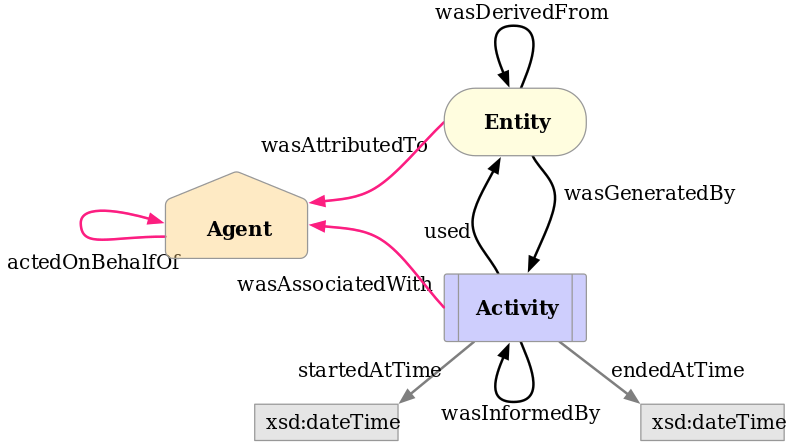
\includegraphics[width=\linewidth]{figs/dag/w3cprov.png}
\caption{Concepts in PROV, copied without modification from \url{https://www.w3.org/TR/2013/REC-prov-o-20130430/}}
\label{fig:prov}
\end{figure}

% <!---"Also note that provenance as modelled in prov is a generic concept, and can represent activities of humans as readily as software processes enacted by workflow engines."--->

\textbf{2016}

% <!-- mentions choice of when to compute/store intermediate result. this is also mentioned in Simmhan et al. 2005--->
Regalia et al. \cite{Regalia2016} propose the \textit{VOLT} language to add provenance on top of \textit{SPARQL} (the W3C standardised query language for semantic databases). \textit{VOLT} works as a proxy, that dynamically generates derived properties on demand, then queries the result using standard \textit{SPARQL} as if the properties had been manually defined. Furthermore it captures provenance. It is demonstrated with a case study of spatial queries to dynamically generate compass direction relations between nearby locations (e.g. A \textit{is east of} B). This is both more accurate and storage efficient than manually defining the compass direction between every possible pair of locations. The system supports provenance in two ways. Firstly, all queries run are serialised as an abstract syntax tree along with their outputs and stored in a temporary \textit{results graph} or persistent \textit{output graph}. This allows the framework to determine whether a cached result is still valid, or whether the inputs have changed and it needs to be recomputed. The user can also perform queries over the results graph itself to query the provenance of a result stored in the results graph (such as which data sources were used, or which functions the query depended on). Secondly, functions in \textit{VOLT} optionally support collection of additional metadata that help the user understand how the result was computed. The authors of \textit{VOLT} provide the example that an operation to sum up attributes from multiple geographic regions would also capture the combined geographic region involved in the calculation as well as any overlap between regions. The user can visualise this metadata to as a form of assurance that the query was calculated as expected (e.g. if visualising the overlap between regions reveals significant overlapping area, this may indicate unintentional double counting when summing up attributes from these regions).

% <!--- notes need for "alignment of our provenance and model graphs with ontologies such as PROV-O [6] and (semantic) workflow models in general" as future work -->
% <!---
% -> https://ieeexplore.ieee.org/document/4404805/ "Examining the Challenges of Scientific Workflows" (overview of unique characteristics of scientific workflows)
% ---->

% \nb{Liming Zhu (Data61) is co-author of \cite{Wu2016}}

D. Wu, L. Zhu (Data61), et al. \cite{Wu2016} describe ``Pipeline61'', a tool for constructing and managing pipelines that contain components that are implemented in different big data frameworks and data stores. While not the main focus of their article, their pipeline is also designed to capture data provenance in a manner that integrates with the need for dependency management and version control of components.

To do this, they capture an \textit{execution trace}, a \textit{dependency tree} and a \textit{data snapshot}. The execution trace captures a DAG of the pipeline each execution. Capturing a separate DAG each execution allows version control of the pipeline itself to deal with configuration changes such as additional inputs or different versions of components. The \textit{execution trace} itself does not include data or source code, so the cost of capturing a complete DAG each execution is minimal. The \textit{dependency tree} captures the dependencies of each component: the environment it depends on, the path to the component source code, and the executions it was used on. The description of the environments is constrained to a set of prespecified labels such as SparkPipe or ShellPipe which are supported by Pipeline61. In their example, the source code of the component is assumed to be a single file, so it is unclear how one would represent components with dependencies on specialised libraries or components that share code with each other. The tracking of the executions the component was run on as part of the dependency tree appears to be redundant considering that this information is also in the execution traces (perhaps the authors intended it as a view rather than a capture of duplicate information); however, exposing this information helps regression test new components against real inputs and outputs fed to the previous version of the component in production. The \textit{data snapshot} captures all inputs to each version of a component, the output, and the execution state (i.e. whether there were any errors). The data captures themselves are identified by the component, component version, and execution trace ID. The use of execution trace ID as part of the data capture ID would seem to prevent the ability to perform an incremental build that can reuse the output of initial stages of the pipeline that haven't changed (perhaps the authors desired the entire pipeline to be rerun each execution due to \textit{non-pure}\footnote{``purity'' is used in the sense of the functional programming paradigm. I.e. a ``pure'' function is like a mathematical function that has no effect other than returning a value in contrast to a ``non-pure'' function that has side-effects that alter the program state.} functions in the pipeline that may generate a different output for the same inputs, interact with an external system, or produce errors\footnote{e.g. errors could result from race conditions in poor concurrent programming implementations, or be induced by spontaneous hardware faults such as ``soft errors'' arising from ionising radiation} that resolve themselves after restarting the process).

\textbf{2017 -- 2019}

% A Templating System to Generate Provenance (published 2018, but was in review since 2016)
As W3C PROV can be tedious and error-prone to generate, Moreau et al. \cite{Moreau2018} describe a templating system to generate valid W3C PROV statements. The templates are expressed as PROV documents containing variables as placeholders. This simplifies the process of modifying an application to output provenance information, as all the application needs to generate is a mapping that binds template variables to values. These bindings are then used by the templating system to expand the templates into full PROV statements (or can be left as is in compressed form).

% PROV2R (2017, but logically flows as a recent development)
Stamatogiannakis et al. \cite{Stamatogiannakis2017} describe ${PROV}_{2R}$, a tool for capture of provenance information on systems where one is using off-the-shelf software, and does not have the ability/resources to modify the software itself to output provenance information. This is achieved by running the whole system within an emulated machine using PANDA \cite{Dolan-Gavitt2015}, which captures a re-playable snapshot of the system along with a log of all non-deterministic operations. These logs can then be replayed with taint-tracking at the desired granularity to determine which inputs affect which outputs. The resultant logs can be exported to W3C PROV and queried.

% https://github.com/moyix/panda/blob/master/docs/manual.md
% "Deterministic record and replay is a technique for capturing the non-deterministic inputs to a system"
